\documentclass[12pt]{article}
%\usepackage[utf8]{inputenc}
\usepackage[french]{babel} 
\usepackage[T1]{fontenc}
\usepackage{graphicx}
\usepackage{xcolor}
\usepackage{lmodern}
\usepackage{array}
\usepackage{float}

%load default definitions 
%%novalidate

\usepackage{tikz}
\usepackage{calc}
\usepackage{booktabs}
%\usepackage{hyperref}

% colors
\definecolor{color1}{HTML}{000060}
%\definecolor{color1}{HTML}{8C260F}
\definecolor{color2}{HTML}{333333}


% fonts
\usepackage{fontspec}
\defaultfontfeatures{Mapping=tex-text}
\setmainfont
[BoldFont=Lato-Bold.ttf,
ItalicFont=Lato-Italic.ttf,
BoldItalicFont=Lato-BoldItalic.ttf]
{Lato-Regular.ttf}
\newfontfamily\headingfont[ItalicFont=Lato-BlackItalic.ttf]{Lato-Black.ttf}
%%%

\usepackage{geometry}
\geometry{a4paper,
hmargin=20mm,vmargin=20mm,
head=15pt,foot=3ex}

\linespread{1.3}

\usepackage[hang]{caption}
\DeclareCaptionFormat{upper}{#1#2\uppercase{#3}\par}
\captionsetup{labelfont={bf,color=color2},textfont={normalsize,color=color2},format = upper,figurename=FIGURE,tablename=TABLE}

%%% fancy sections
\usepackage{titlesec}
%\titleformat{\chapter}{\headingfont\LARGE\bfseries\scshape\color{color1}}{\thechapter}{1em}{}[\titlerule]
\titleformat{\section}{\color{color1}\headingfont\Large\bfseries\uppercase}{\thesection}{1em}{}[\titlerule]
\titleformat{\subsection}{\color{color1}\headingfont\large\bfseries\uppercase}{\thesubsection}{1em}{}
\titleformat{\subsubsection}{\color{color1}\headingfont\bfseries\uppercase}{\thesubsubsection}{1em}{}
%%%

% head and foot
\usepackage{fancyhdr}
\pagestyle{fancy}
\lhead{}
\chead{}
\makeatletter
\rhead{\color{color2}\@date}
\makeatother
\newlength{\myheight}
\lfoot{
\settoheight{\myheight}{\thepage}
\raisebox{-2ex-0.5\myheight}{
\includegraphics[height=4ex]{logo}}
}
\cfoot{\color{color2} Projet adenome-pro 2017/2018 }
\rfoot{\color{color2}\thepage}
\renewcommand\headrulewidth{0pt}
\renewcommand\footrulewidth{0pt}

%%% picture on cover page
\usepackage{eso-pic}
\newcommand\BackgroundPic{%
\put(0,0){%
\parbox[b][\paperheight]{\paperwidth}{%
\vfill
\centering

\includegraphics[width=\paperwidth,height=\paperheight,%
keepaspectratio]{logo}%
\vfill
}}}
%%%
% custom titlepage
\makeatletter
\renewcommand{\maketitle}{
\thispagestyle{empty}
\AddToShipoutPicture*{\BackgroundPic}
\ClearShipoutPicture
%
\phantom{a}
\vfill
\phantom{a}\hfill
\begin{tabular}[c]{@{}p{0.7\textwidth}@{}}
      \color{black}\headingfont\LARGE\@title\\[1em]
      \color{black}\headingfont\Large\@author\\[2em]
\end{tabular}
%
\clearpage
}
\makeatother
%%%


%%% fancy boxes
\usepackage{tcolorbox}
\usepackage{wrapfig}
\def\fullboxbegin{
\bigskip
\begin{tcolorbox}[colback=color1,colframe=color1,coltext=white,arc=0mm,boxrule=0pt]
}
\def\fullboxend{\end{tcolorbox}\medskip}
%
\def\leftboxbegin{
\begin{wrapfigure}{l}{0.5\textwidth}
\begin{tcolorbox}[colback=color1,colframe=color1,coltext=white,arc=0mm,boxrule=0pt]
}
\def\leftboxend{
\end{tcolorbox}
\end{wrapfigure}
}
%
\def\rightboxbegin{
\begin{wrapfigure}{r}{0.5\textwidth}
\begin{tcolorbox}[colback=color1,colframe=color1,coltext=white,arc=0mm,boxrule=0pt]
}
\def\rightboxend{
\end{tcolorbox}
\end{wrapfigure}
}
%
\newcounter{frames}
\def\frameboxbegin#1{
\bigskip
\refstepcounter{frames}
\begin{tcolorbox}[colback=white,colframe=color1,arc=0mm,title={\MakeUppercase{\textbf{Frame \arabic{frames}}: #1}}]
}
\def\frameboxend{
\end{tcolorbox}
}
%%%

%################################################################
% HEADER
%################################################################
\title{Projet  adenome-pros}
\author{Guillaume Morin, Frédéric Saunier}
\date{\today}
\begin{document}
\maketitle
\tableofcontents
\clearpage


%################################################################
% DOCUMENT BEGIN 
%################################################################

%introduction
\section{Introduction}

Cette étude porte sur 3 bases de données mediacles VAPOR, RTUPB et VPPBS. Ces trois bases fournissent un ensemble de données pré et post opératoire pour un ensemble de patients utilisant l'un des trois traitements. Sachant que les données post opératoires sont fournies sous forme d’observation sur des intervalles de temps distincts. 


\newcolumntype{M}[1]{>{\raggedright}m{#1}}
\begin{table}[!h]
\centering
\caption{Glossaire}
\begin{tabular}{|l|p{11cm}|}
\toprule
Variable   & Déscription    \tabularnewline              \\
\midrule
Age (ans)     & Age du  patient                \\ 
\hline
Comorbidité CardioVx     &  Présence de maladies  associées cardiaque ou vasculaire tel que  l'hypertension arterielle      \\
\hline
Durée traitement médical (mois)  &   N/A       \\
\hline
Porteur de sonde & le patient a une sonde urinaire avant l'intervention      \\
\hline
IPSS P.O     & International prostatic syptome score PRE OPERATOIRE = plus il est elevé plus le patient est gené          \\
\hline
QoL P.O   &  Score de qualité de vie PRE OPERATOIRE = plus il est elevé plus le patient est insatisfait                          \\
\hline
Qmax P.O (ml/s)    & Débit maximal urinaire PRE OPERATOIRE = plus il est elevé, plus la miciton est de bonne qualité 	  \\
\hline
PSA (ng/ml)    & N/A  \\
\hline
Volume prostatique (ml)    & N/A  \\
\hline
RPM     & Residu post mictionnel = quantité d'urine retrouvé dans vessie après une miction, à l'état normal elle est de 0    \\
\hline
Indication  & N/A                           \\
\hline
Anesthésie     & N/A                           \\
\hline
Evenement H.D    & Evenement hémodynamique pendant l'intervention = perturbation de la tension arterielle durant l'intervention   \\
\hline
Transfusion PerO  & Si oui ou non le patient a eu une transfusion pendant l'intervention                           \\
\hline
Temps OP     & Temps opératoire                          \\
\hline
Volume résequé (ml)   & N/A                           \\
\hline
Délai ablation (jours)l)   & Délai d'ablation de la sonde urinaire après l'intervention 	  \\
\hline
caillotage & N/A                           \\
\hline
reprise au bloc  & N/A                           \\
\bottomrule
\end{tabular}
\end{table}

	 	 	 			
\newpage

%###############################################################
%Analyse descriptive 
%###############################################################
\section{Analyse déscriptive}

%vue d'ensemble 
\subsection{Vue génerale}
  %"###############################################
%
% Vue d'ensemble / générale 
%
%###############################################

RTUPB, VPPBS et VAPOR sont trois bases d'observations contenant respectivement 36, 32 et 40 observations (patients) avec une répartition en âge suivante : 

\begin{figure}[h]
    \begin{minipage}[c]{.46\linewidth}
        \centering
        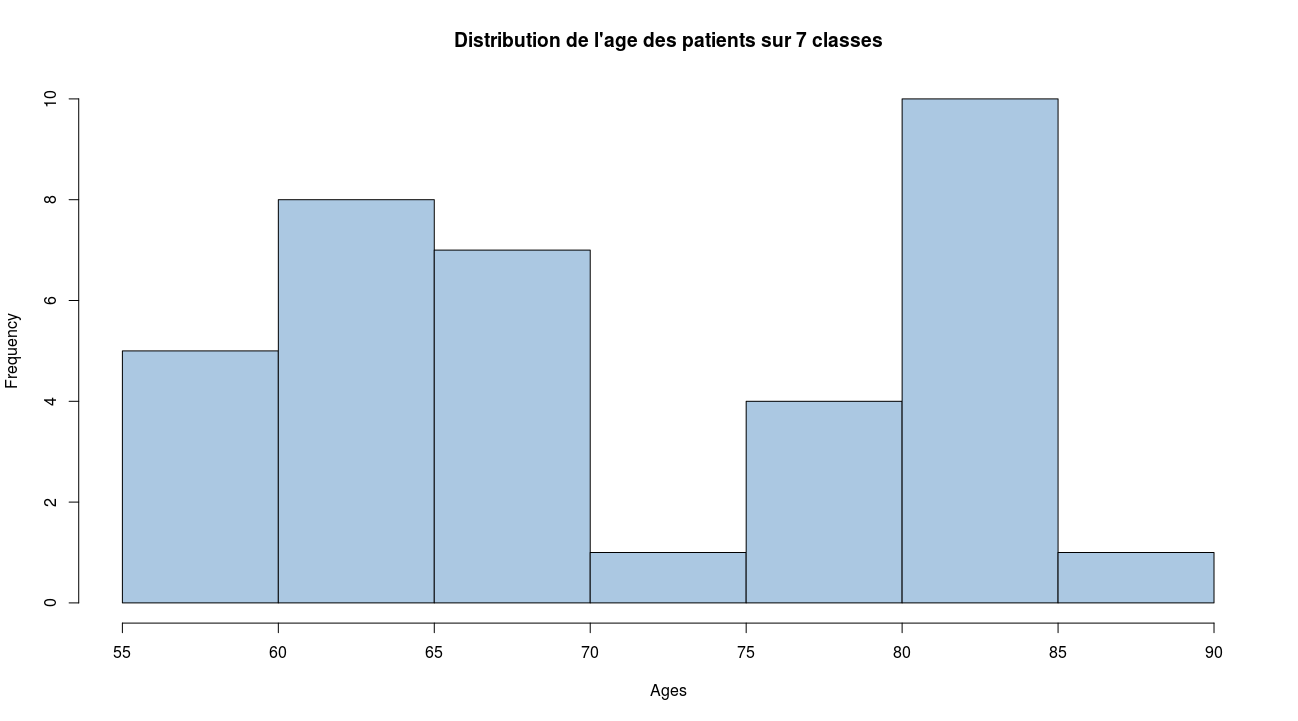
\includegraphics[width=1\textwidth]{../Fig/RTUPB/rtupb-age-frequency}
        \caption{RTUPB}
    \end{minipage}
    \hfill%
    \begin{minipage}[c]{.46\linewidth}
        \centering
        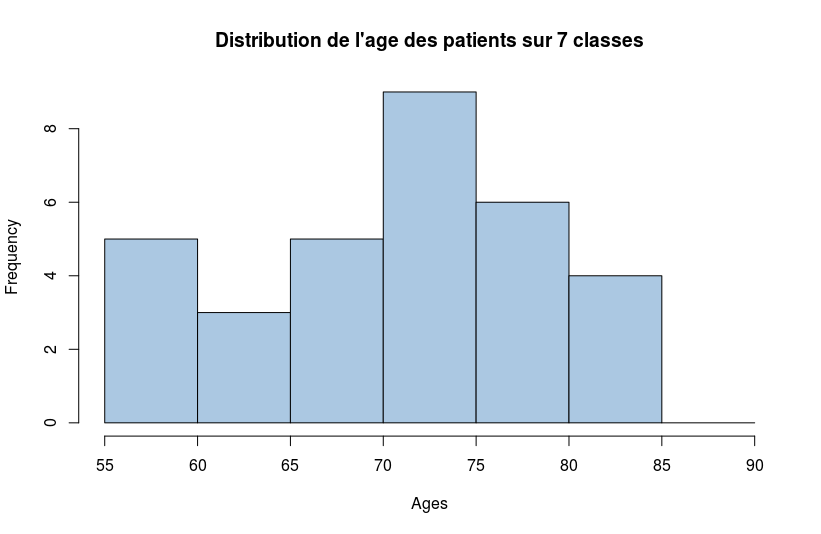
\includegraphics[width=1\textwidth]{../Fig/VPPBS/vppbs-age-frequency.png}
        \caption{VPPBS}
    \end{minipage}
\end{figure}


\begin{figure}[H]
\centering
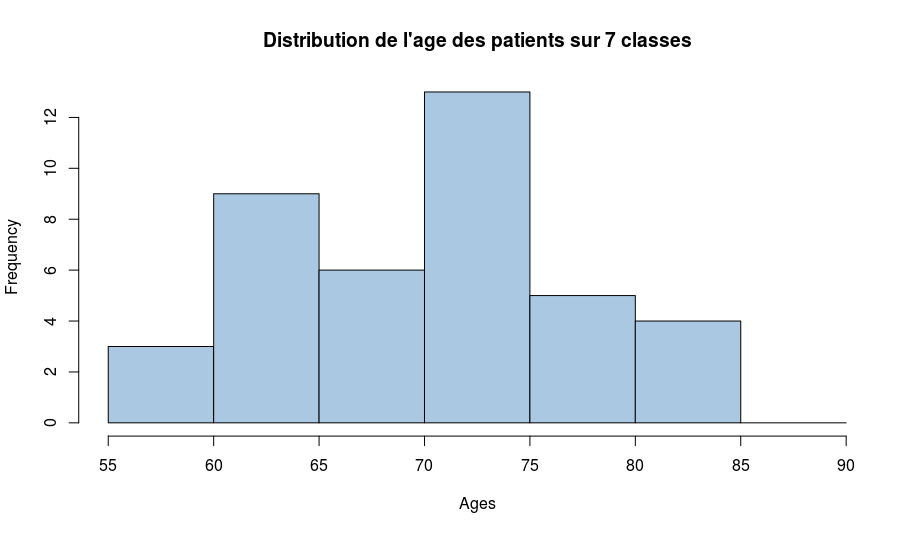
\includegraphics[width=0.50\textwidth]{../Fig/VAPOR/vapor-age-frequency}
\caption{VAPOR}
\end{figure}


%
%##########################
%# CONCLUSION
%##########################

%corrélations 
\subsection{Corrélation variables pre-opératoires}
  %"###############################################
%
% Corrélations 
%
%###############################################

Ici nous souhaitons mettre en évidence les corrélations possibles.
Nous limitons l’étude sur les tableaux post-opératoires des techniques RTUBD VPPBS et VAPOR contenant 
aussi les variables IPSS Qol et Qmax.
De même, certaines dimentions sont invariantes pour une technique donnée, nous avons supprimé celles-ci lors de la création 
de la matrice de corrélation et son corralélograme associé.

\begin{figure}[H]
\centering
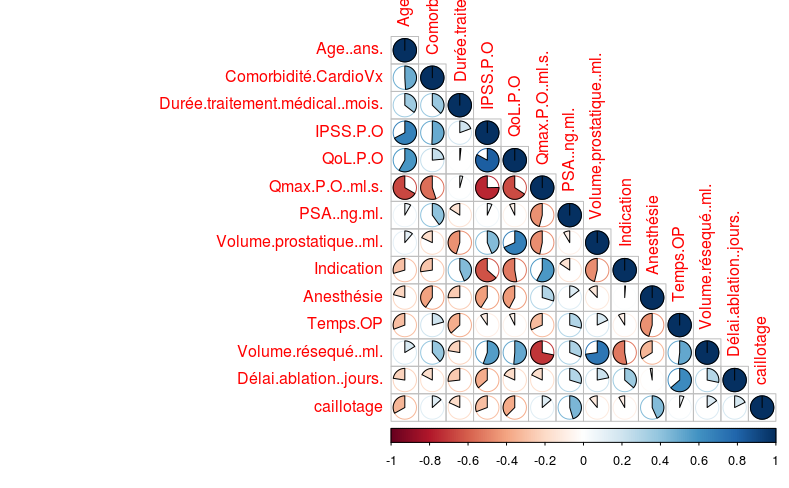
\includegraphics[width=0.75\textwidth]{../Fig/RTUPB/rtupb-corr-matrice-pie}
\caption{Matrice corrélation RTUBP}
\end{figure}

\begin{figure}[H]
\centering
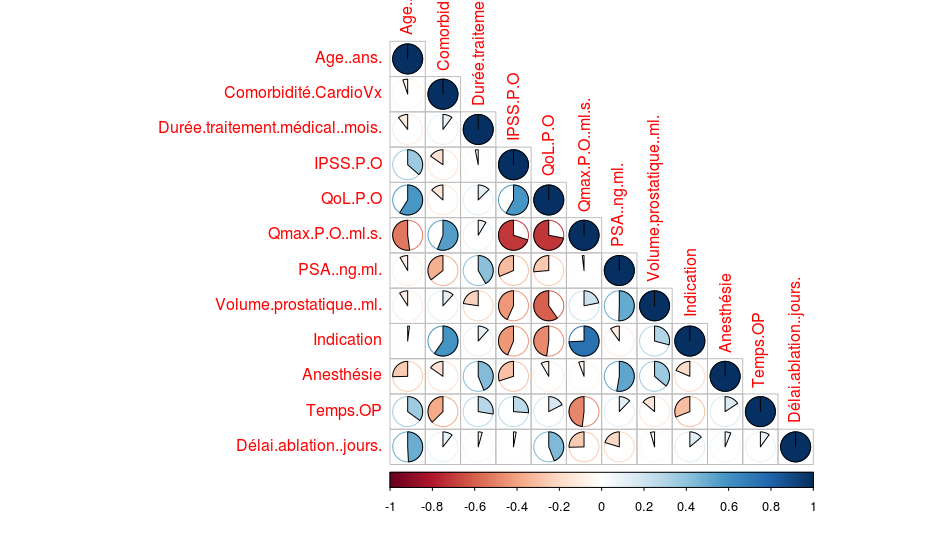
\includegraphics[width=0.75\textwidth]{../Fig/VPPBS/vppbs-corr-matrice-pie}
\caption{Matrice corrélation VPPBS}
\end{figure}

\begin{figure}[H]
\centering
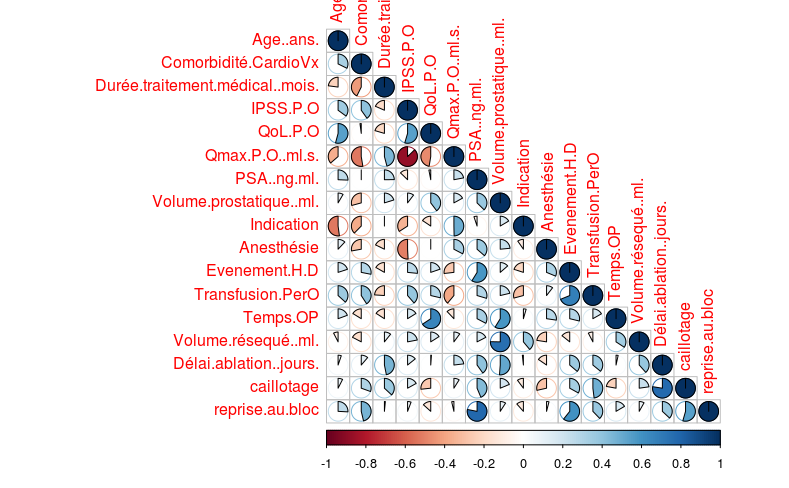
\includegraphics[width=0.75\textwidth]{../Fig/VAPOR/vapor-corr-matrice-pie}
\caption{Matrice corrélation VAPOR}
\end{figure}


Les variables  \emph{IPSS P.O} et   \emph{QoL P.O}  semblent avoir une corrélation qui peut sembler logique à la connaissance du fait qu’elles représentent pour l’une un indicateur de gène et pour l’autre un indicateur une qualité de vie post opératoire, même si c’est nettement plus marqué dans le cas de le panel des patients RTUBP. De même  pour les variables \emph{Volume prostatique} et \emph{Volume réséqué}. Aussi nous avons une corrélation \textbf{negative} intéressante entre le \emph{IPSS P.O} et le \emph{QMAX PO (ml/s)} (plus le patient à un QMax élevé moins il semble gêné alors que IPSS croît avec la gêne). 




%\begin{figure}[h]
%    \begin{minipage}[c]{.46\linewidth}
%        \centering
%        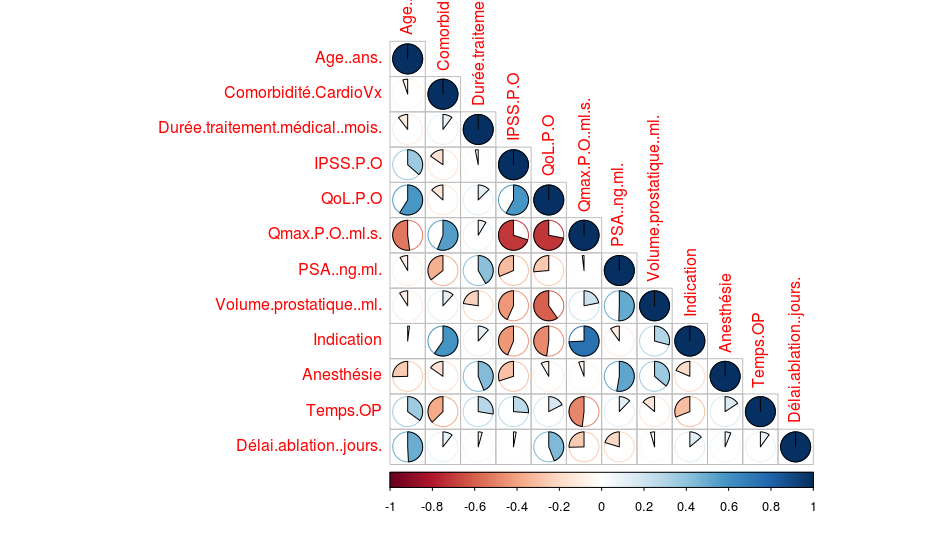
\includegraphics[width=1\textwidth]{../Fig/VPPBS/vppbs-corr-matrice-pie}
%        \caption{Légende}
%    \end{minipage}
%    \hfill%
%    \begin{minipage}[c]{.46\linewidth}
%        \centering
%        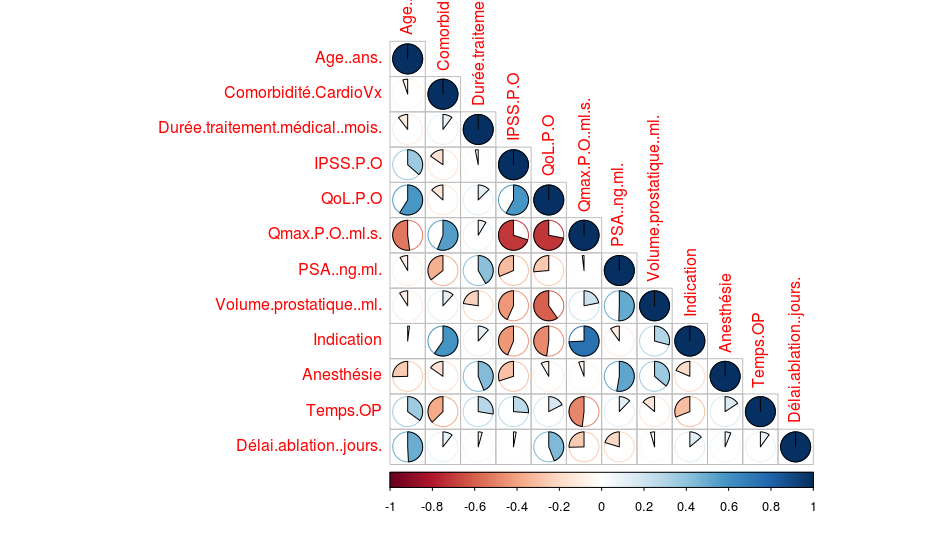
\includegraphics[width=1\textwidth]{../Fig/VPPBS/vppbs-corr-matrice-pie}
%        \caption{Légende}
%    \end{minipage}
%\end{figure}





%
%##########################
%# CONCLUSION
%##########################

\subsection{Distribution/évolution des données post-opératoires}
  %"###############################################
%
% IPSS
%
%###############################################

Dans l’analyse suivante nous souhaitons observer la distribution des variables IPSS Qol Et Qmax sur les différentes itérations temporelles fournies. L’objectif est de voir (pour l’ensemble des patients utilisant l’une des trois techniques ) comment cette distribution évolue.) 

\subsubsection{IPSS sur 18 mois }

RTUPB est une table composée de 36 patients. 
	
\begin{figure}[H]
\centering
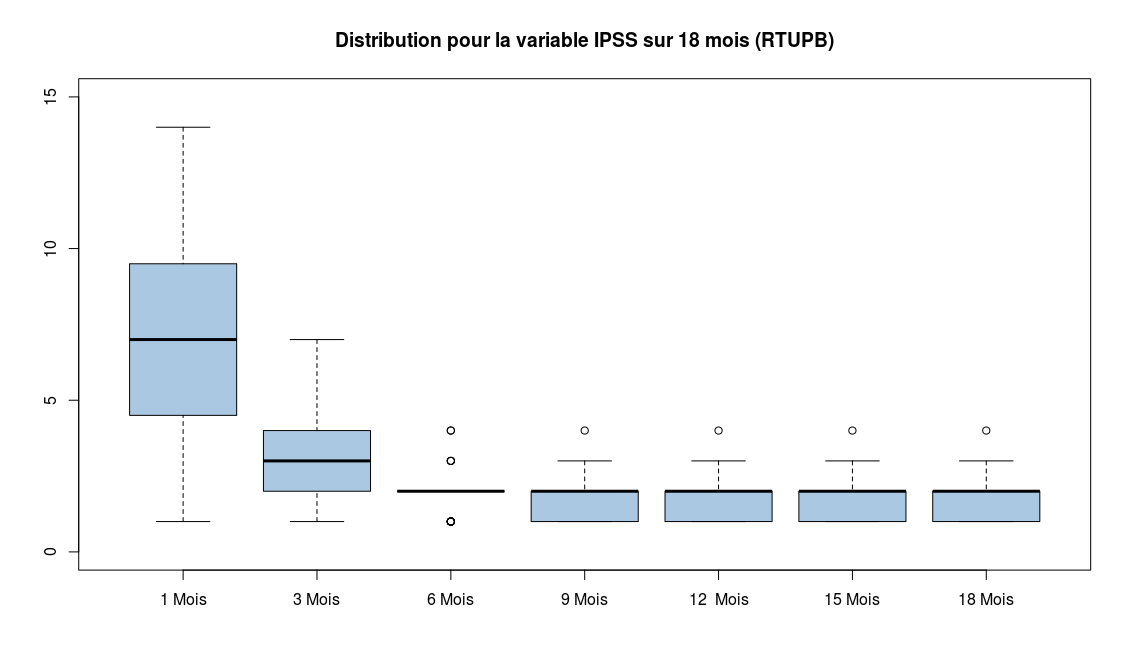
\includegraphics[width=0.75\textwidth]{../Fig/RTUPB/rtupb-boxplot-post-ipss}
\caption{RTUPB / IPSS sur 18 mois}
\end{figure}	
	
\begin{figure}[H]
\centering
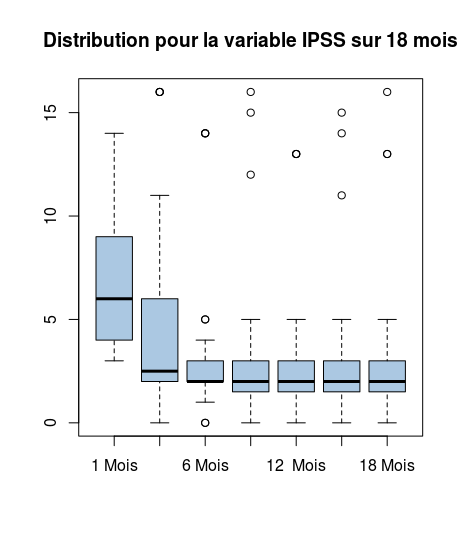
\includegraphics[width=0.75\textwidth]{../Fig/VPPBS/vppbs-boxplot-post-ipss}
\caption{VPPBS/IPSS sur 18 mois}
\end{figure}


\begin{figure}[H]
\centering
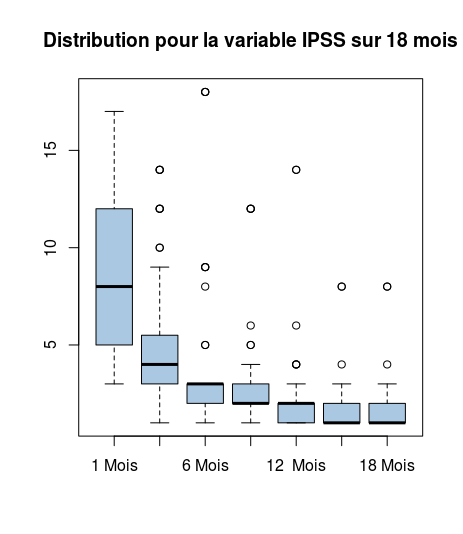
\includegraphics[width=0.75\textwidth]{../Fig/VAPOR/vapor-boxplot-post-ipss}
\caption{VAPOR/IPSS}
\end{figure}

%
%##########################
%# CONCLUSION
%##########################

Pour IPSS, l’on observe pour les trois techniques une décroissance de la valeur médiane dés le troisièmes mois. Dans le cadre de VAPOR et VPPBS, certains « outliers » sont présents (et ce sur l’ensemble des itérations dans le cadre de VPPBS ces « outliers » ont encore des valeurs très fortes même à partir du 18 mois.  RTUPB  semble avoir une variance homogène à partir du 9 ieme mois. Si VAPOR laisse apparaître des « ouliers », la valeur médiane termine plus bas que les deux autres techniques. 

  %"###############################################
%
% Qol 
%
%###############################################


\subsubsection{Qol sur 18 mois }

\begin{figure}[H]
\centering
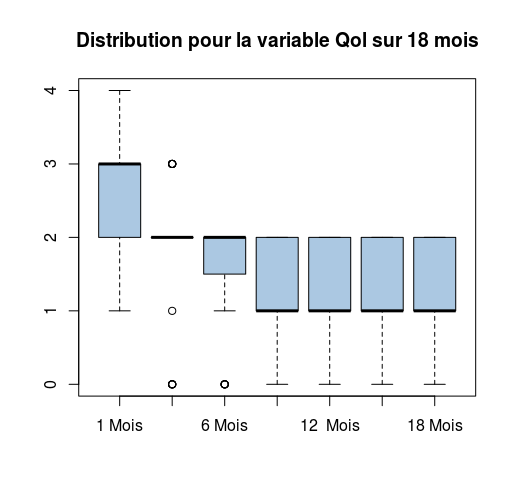
\includegraphics[width=0.75\textwidth]{../Fig/RTUPB/rtupb-boxplot-post-Qol}
\caption{RTUPB / Qol sur 18 mois}
\end{figure}	
	
\begin{figure}[H]
\centering
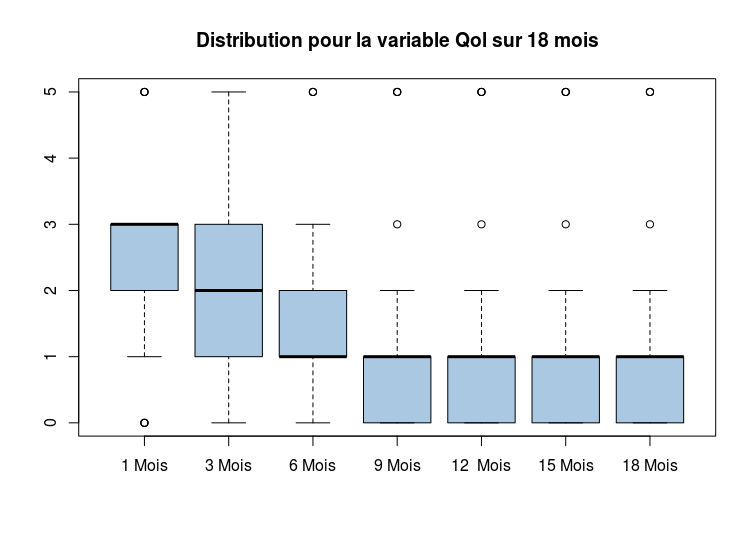
\includegraphics[width=0.75\textwidth]{../Fig/VPPBS/vppbs-boxplot-post-Qol}
\caption{VPPBS / Qol sur 18 mois}
\end{figure}	
	
	
\begin{figure}[H]
\centering
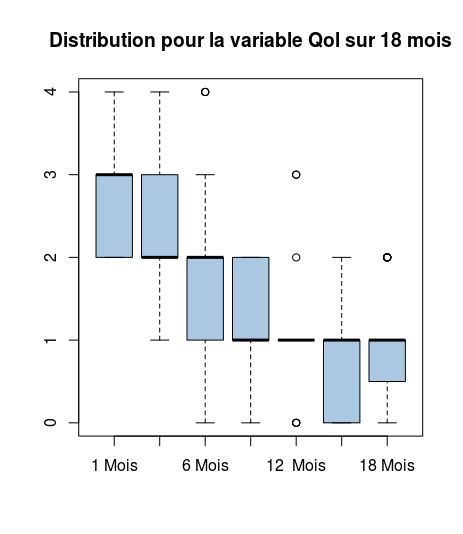
\includegraphics[width=0.75\textwidth]{../Fig/VAPOR/vapor-boxplot-post-Qol}
\caption{VAPOR / Qol sur 18 mois}
\end{figure}	
	


%
%##########################
%# CONCLUSION
%##########################
  %"###############################################
%
% Qmax
%
%###############################################

\subsubsection{Qmax sur 18 mois }

\begin{figure}[H]
\centering
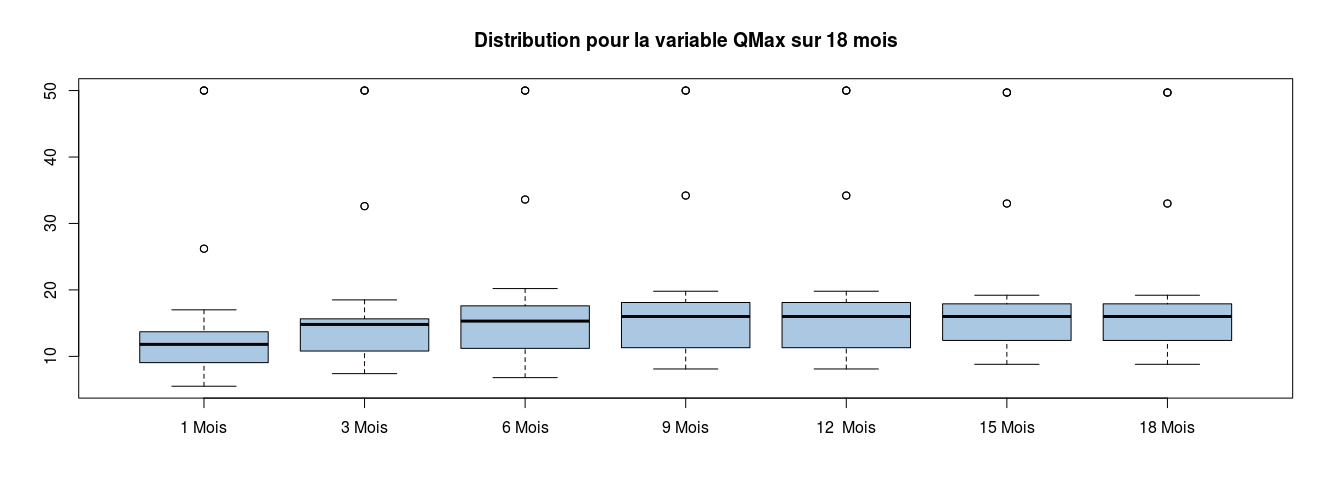
\includegraphics[width=0.75\textwidth]{../Fig/RTUPB/rtupb-boxplot-post-Qmax}
\caption{RTUPB / Qmax sur 18 mois}
\end{figure}	
	
\begin{figure}[H]
\centering
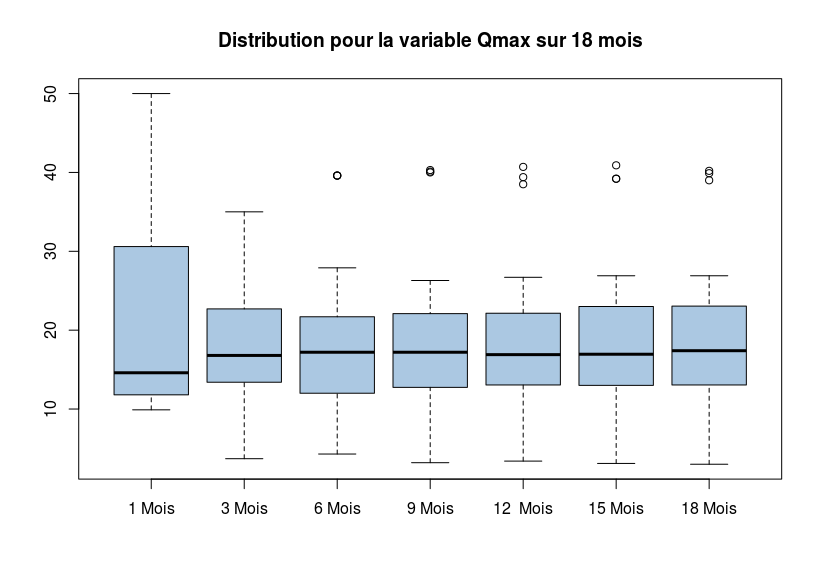
\includegraphics[width=0.75\textwidth]{../Fig/VPPBS/vppbs-boxplot-post-Qmax}
\caption{VPPBS/Qmax sur 18 mois}
\end{figure}


\begin{figure}[H]
\centering
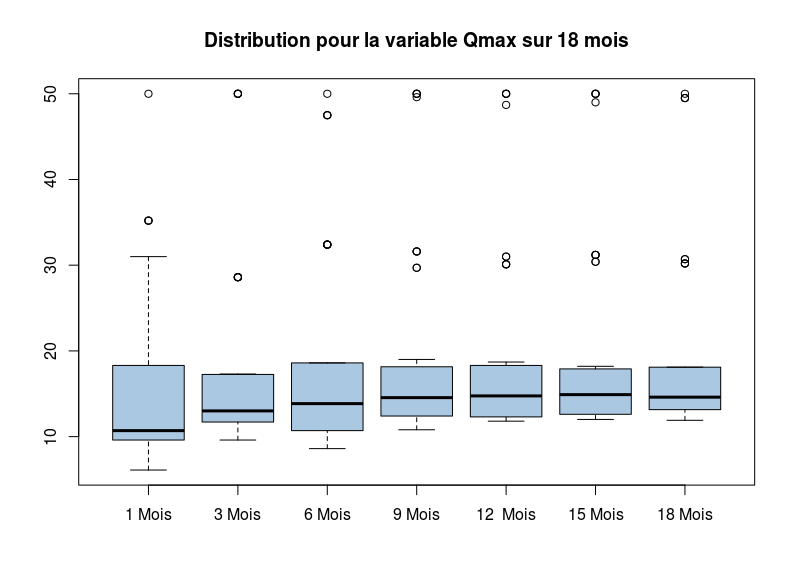
\includegraphics[width=0.75\textwidth]{../Fig/VAPOR/vapor-boxplot-post-Qmax}
\caption{VAPOR/Qmax}
\end{figure}

%
%##########################
%# CONCLUSION
%##########################

RTUPB semble être le plus constant, VPPBS permet d’obtenir de meilleurs résultats sur le Qmax (augmentation) avec des cas extrêmes plus élevés. VAPOR obtient des résultats médians proches de RTUPB mais avec des cas extrêmes plus élevés comparativement aux trois techniques.   
\newpage



%###############################################################
%Classification profils pre Operatoir  
%###############################################################

\section{Classification profils pre-opératoires}

Dans le cadre de la classification nous avons observés quelques doublons, nous avons choisi de les supprimer 
du moins dans cette premiere phase. 


%vue d'ensemble 
\subsection{CAH / PAM RTUPB }
  %"###############################################
%
% Classification RTUPB pre 
%
%###############################################

\begin{figure}[H]
\centering
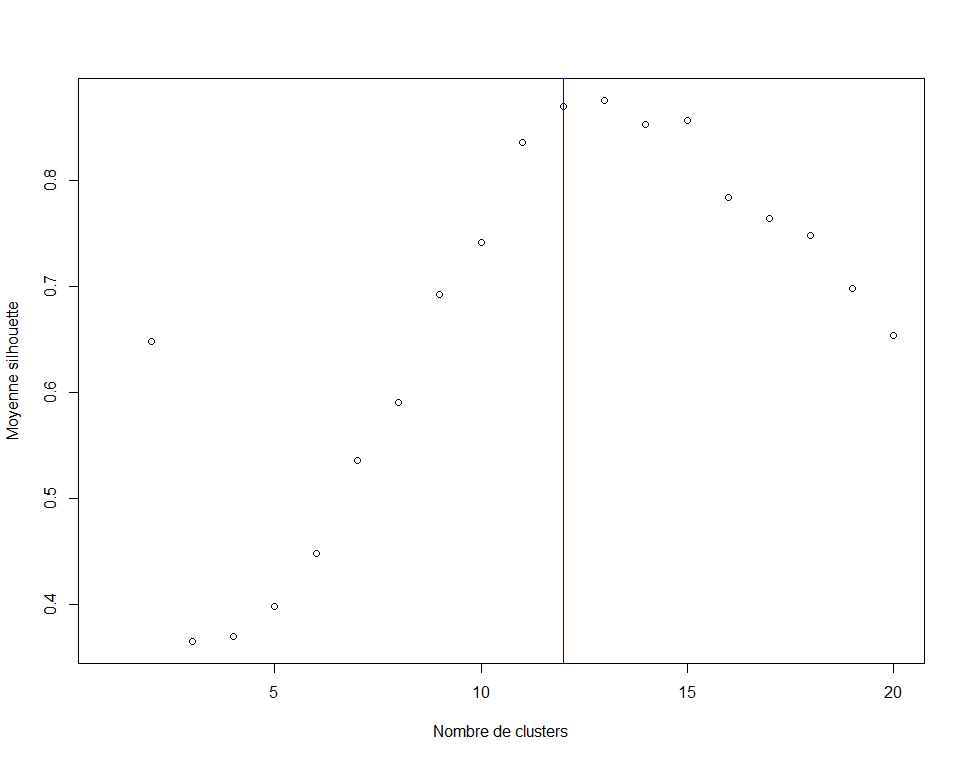
\includegraphics[width=0.90\textwidth]{../Fig/RTUPB/rtupb-elbow-pre.png}
\caption{RTUPB Maximise nb cluster / bonne classification}
\end{figure}

\begin{figure}[H]
\centering
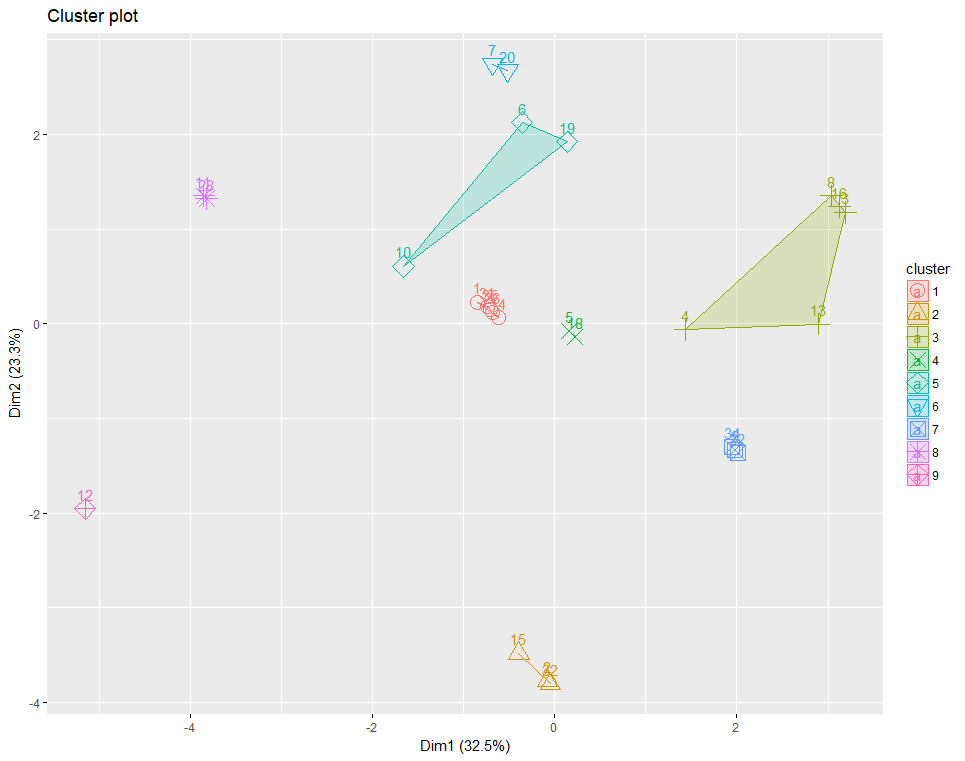
\includegraphics[width=0.90\textwidth]{../Fig/RTUPB/rtupb-pam-k12.png}
\caption{RTUPB Nuage de points / clusters PAM k=12 }
\end{figure}

\begin{figure}[H]
\centering
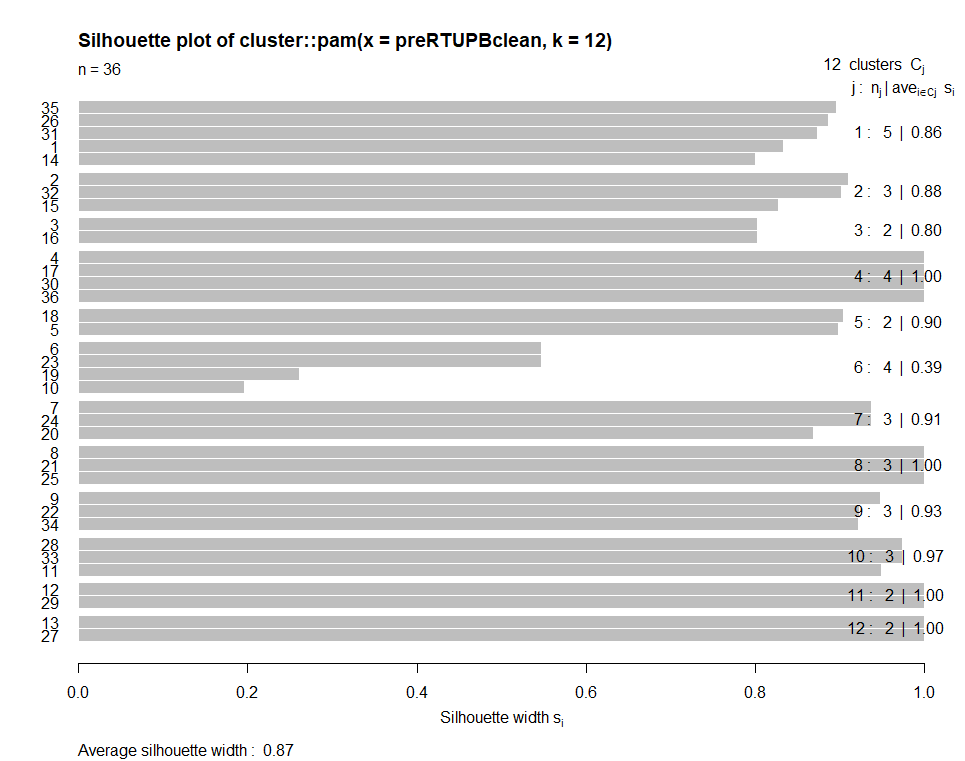
\includegraphics[width=0.90\textwidth]{../Fig/RTUPB/rtupb-sil-k12-pre.png}
\caption{RTUPB silhouette / clusters PAM k=12 }
\end{figure}

\begin{figure}[H]
\centering
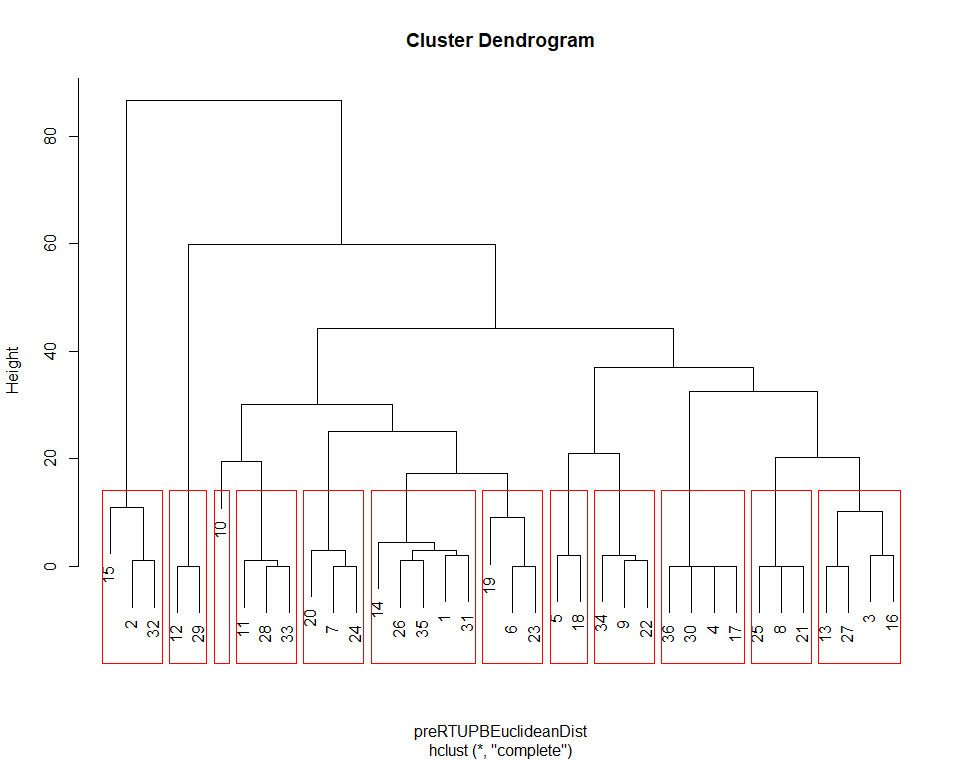
\includegraphics[width=0.90\textwidth]{../Fig/RTUPB/rtupb-cah-k12-pre.png}
\caption{RTUPB CAH séparation en k=12 }
\end{figure}


%"###############################################
%
% Interpretation des trois figures RTUPB pre 
%
%#############################################

Lors de notre analyse nous avons observé qu'il existait un ensemble d'individus similaires (ensemble des valeurs
identiques au relevé prés) ce qui s'observe dans la construction de certains clusters avec une valeur de qualité 
intra-cluster très forte en forgeant de petits clusters. Nous reviendrons sur ce point dans le rapprochement de ces
profils avec les profils de guérison ultérieurement. Nous avons estimé à 12 le nombre de clusters suivant la variation 
de la qualité globale  du cluster réalisé à partir de PAM. 

\textbf{Patients medoids 35, 2 ,16 ,36, 18, 23 ,24 ,25, 9, 33, 29 , 27}


%\begin{figure}[h]
%    \begin{minipage}[c]{.46\linewidth}
%        \centering
%        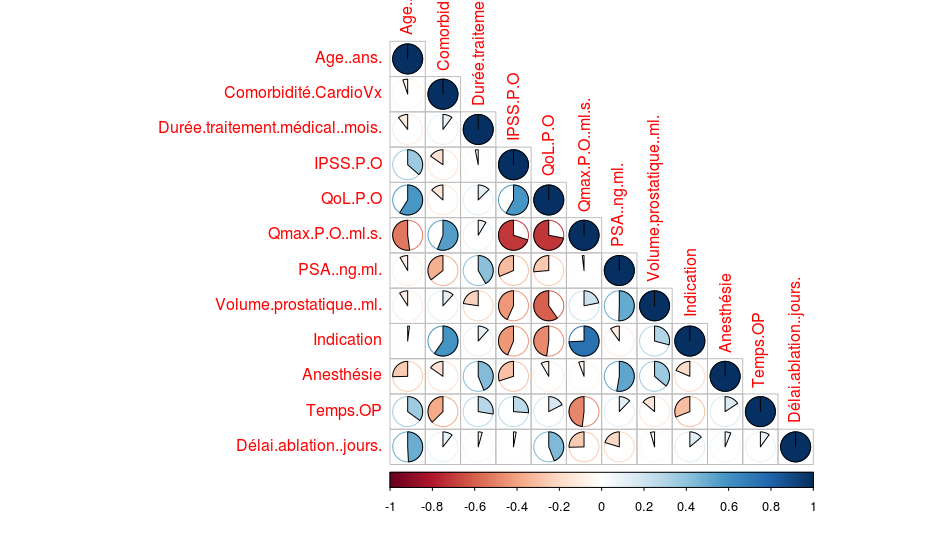
\includegraphics[width=1\textwidth]{../Fig/VPPBS/vppbs-corr-matrice-pie}
%        \caption{Légende}
%    \end{minipage}
%    \hfill%
%    \begin{minipage}[c]{.46\linewidth}
%        \centering
%        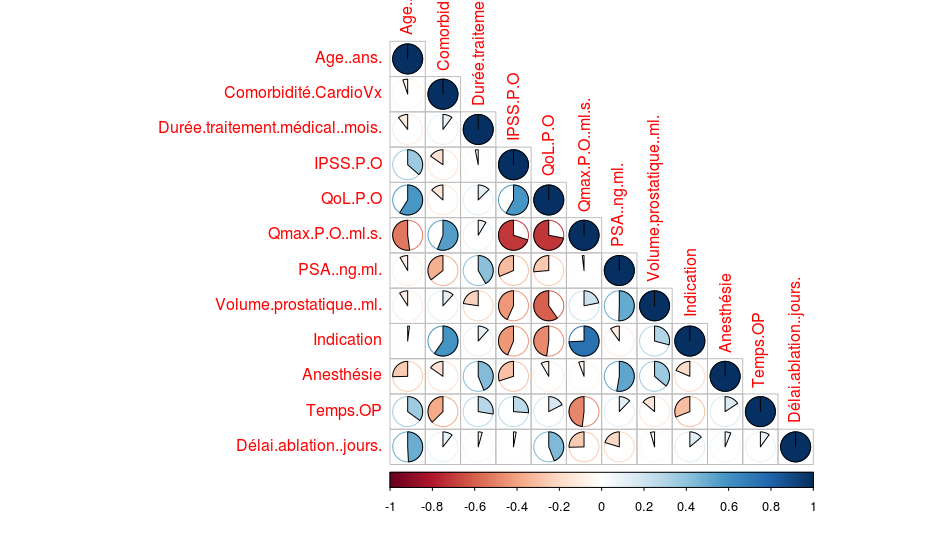
\includegraphics[width=1\textwidth]{../Fig/VPPBS/vppbs-corr-matrice-pie}
%        \caption{Légende}
%    \end{minipage}
%\end{figure}





%
%##########################
%# CONCLUSION
%##########################
  



%\section{Classification des profils pre op.}
%%###############################################
%# RTUPB
%###############################################
\subsection{Extraction des profils pour RTUPBS}

\subsubsection{QMax sur 12 mois}


%###############################################
%# RTUPBS
%###############################################
\subsection{Extraction des profils pour RTUPBS}

\subsubsection{QMax sur 12 mois}



%###############################################
%#QMAX 12 mois 
%###############################################
\subsection{Extraction des profils pour RTUPBS}

\subsubsection{Conclusion}
%\newpage



%\subsubsection{First subsubsection}
%\begin{figure}[!h]
%\centering
%\includegraphics[width=0.5\textwidth]{sky.jpg}
%\caption{The sky is the limit.}
%\end{figure}


%%%\lipsum[1]
%\begin{table}[!h]
%\centering
%\caption{Sample table.}
%\begin{tabular}{cccc}
%\toprule
%Value 1 & Value 2 & Value 3 & Value 4\\
%\midrule
% odd     & odd   & odd & 1.00 \\
% even    & even  & even& 1.00 \\
% odd     & odd   & odd & 1.00 \\
 %even    & even  & even& 1.00 \\
%\bottomrule
%\end{tabular}
%\end{table}
%\frameboxbegin{Sample frame}
%\frameboxend

\end{document}          
